\documentclass[t]{beamer}
\usepackage[ngerman]{babel}
\usepackage{worksheet}

\begin{document}
	\author{L. Bung}
	\title{Vom ER-Modell zum Relationenmodell}
	\date{16.10.2025}
	\begin{frame}
		\titlepage
	\end{frame}
	\begin{frame}{Literatursuche bei der UB Freiburg}
		\begin{figure}[H]
			\centering
			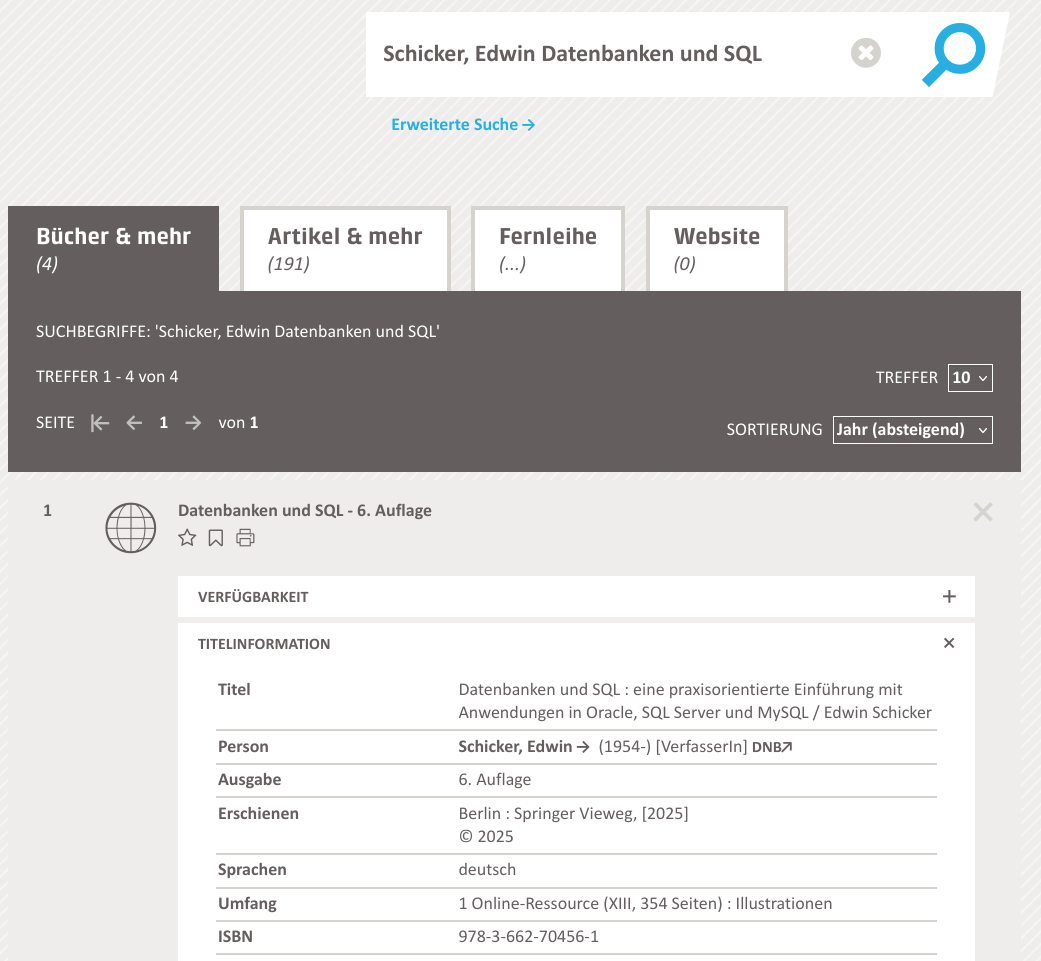
\includegraphics[width=.8\textwidth]{UB_Freiburg_suche.png}
		\end{figure}
	\end{frame}
	\begin{frame}{Situation}
		\begin{figure}[H]
			\centering
			\scalebox{.7}{
			\begin{tikzpicture}[node distance=3cm]
				\node[entity] (autor) {Autor};
				\node[attribute] (autorid) [left of=autor] {\underline{AutorID}} edge (autor);
				\node[attribute] (autorname) [above right of=autor] {Name} edge (autor);
				\node[attribute] (geburtsdatum) [above left of=autor] {Geburtsdatum} edge (autor);
				\node[relationship] (schreibt) [right of=autor] {schreibt} edge node[above]{$n$} (autor);
				\node[entity] (publikation) [right of=schreibt] {Publikation} edge node[above]{$m$} (schreibt);
				\node[attribute] (publikationsid) [above right of=publikation] {\underline{PublikationsID}} edge (publikation);
				\node[attribute] (publikationstitel) [right of=publikation] {Titel} edge (publikation);
				\node[relationship] (veröffentlicht) [below of=publikation, align=center] {veröffentlicht\\ in} edge node[left]{$n$} (publikation);
				\node[entity] (journal) [below of=veröffentlicht] {Journal} edge node[left]{$1$} (veröffentlicht);
				\node[attribute] (journalid) [right of=journal] {\underline{JournalID}} edge (journal);
				\node[attribute] (journaltitel) [below right of=journal] {Titel} edge (journal);
				\node[relationship] (hat) [below of=autor] {hat} edge node[right]{$1$} (autor);
				\node[entity] (login) [below of=hat] {Login} edge node[right]{$1$} (hat);
				\node[attribute] (kontonummer) [below left of=login] {\underline{Kontonummer}} edge (login);
				\node[attribute] (passwort) [below right of=login] {Passwort} edge (login);
			\end{tikzpicture}
			}
		\end{figure}
	\end{frame}
	\begin{frame}{Relationenmodell: Relationen als Tabelle}
		\begin{itemize}
			\item \textbf{1:1-Relation}
			\begin{itemize}
				\item Fremdschlüssel bei einer der beiden Tabellen
				\item Welche Tabelle: egal!
			\end{itemize}
			\item \textbf{1:n-Relation}
			\begin{itemize}
				\item Fremdschlüssel auf der n-Seite
				\item Verweis auf Primärschlüssel der 1-Seite
			\end{itemize}
			\item \textbf{n:m-Relation}
			\begin{itemize}
				\item Extra-Tabelle nötig!
				\item Dort: zwei Fremdschlüssel
				\item Verweis auf Primärschlüssel der n- und m-Seite
			\end{itemize}
		\end{itemize}
	\end{frame}
	\begin{frame}{Relationenschreibweise}
		\begin{itemize}
			\item Schreibweise, aus der die Tabellen klar hervorgehen
			\item Tabellenname und alle Spaltennamen angegeben
			\item Primär- und Fremdschlüssel gekennzeichnet
		\end{itemize}
		
		Beispiel:
		
		\texttt{Kunde(\underline{KundenID}, Name, Geburtsdatum, \dashuline{Ausweisnummer})}
		
		\begin{itemize}
			\item \texttt{\underline{KundenID}}: Primärschlüssel, unterstrichen
			\item \texttt{\dashuline{Ausweisnummer}}: Fremdschlüssel, gestrichelt unterstrichen (manchmal kursiv)
			\item Fremdschlüssel verweist auf Primärschlüssel einer anderen Tabelle
		\end{itemize}
	\end{frame}
\end{document}